%\documentclass[A4,12pt]{article}
\documentclass[letterpaper,12pt]{article}
\usepackage{epsfig}
\usepackage{float}
\usepackage{amssymb,amsmath,latexsym}
\usepackage[labelformat=empty]{caption}
\usepackage{color}
%\usepackage[abs]{overpic}

\usepackage{graphicx}
\usepackage{epstopdf}

\usepackage{tikz}
\usetikzlibrary{arrows}
\usetikzlibrary{calc}
\usetikzlibrary{scopes}
\usetikzlibrary{shadows}
\usetikzlibrary{chains}
%\usetikzlibrary{shadows.blur}

\topmargin      0in 
\textheight     9.0in 
\headheight     -0.0in 
\headsep        0in
\textwidth      6.5in 
\oddsidemargin  0in 
\evensidemargin 0in
\parskip        0pt

\newcommand{\slfrac}[2]{\left.#1\middle/#2\right.}
\newcommand{\bm}    [1]{\mbox{\boldmath $#1$}}

\newtheorem{thm}           {Theorem}
\newtheorem{lemma}    [thm]{Lemma}
\newtheorem{prop}     [thm]{Proposition}
\newtheorem{property} [thm]{Property}
\newtheorem{defin}    [thm]{Definition}
\newtheorem{corollary}     {Corollary}

\begin{document}
  \noindent COM 5165 Multiple Antenna Communication \hfill 113064501 Chun-Ting Lin\\

  \begin{center}
    {\bf \large  Homework III}
  \end{center}


  %--------------------------------------------------------------
  \begin{enumerate}
    \item[{\bf 2. }]  \textbf{$\epsilon$-outage probability} \hfill \\
      The simulation consists of two parts:
\vspace{-5pt}
\begin{itemize}
	\item[(1)] \textbf{Generate theoretical curve \hfill \\}
	Generate the theoretical curve under different $L$ and SNR by
	\begin{equation*}
		C_{\epsilon, \text{theoretical}} = \log\left(1 + F^{-1}(1-\epsilon) \, \text{SNR}\right)
	\end{equation*}
	where $F(x) = P\left(\|h\|^{2} > x\right)$ and $\|h\|^{2}$ is chi-square distribution with $2L$ degrees of freedom.
	\item[(2)] \textbf{Generate Simulated curve \hfill \\}
	To generate the simulated curve, recall the definition of $\epsilon$-outage probability:
	\begin{equation*}
		\epsilon\left(C\right) = P\left(\log(1 + \|h\|^{2} \, \text{SNR}) < C\right)
	\end{equation*} 
	Given $\epsilon$, $L$, and SNR, we first generate a large number ($N = 10^6$) of channel 
	realizations from a chi-square distribution with $2L$ degrees of freedom. Calculate 
	$\log(1 + \|h\|^{2} \, \text{SNR})$ for each realization and sort them into nondecreasing 
	order. Let $k = N\epsilon$, and pick the $k$th smallest value from the sorted data, which
	 is then the simulated result.

\end{itemize}

The comparison between theoretical computation and simulation is shown below. Solid lines 
represent the theoretical result and marked points show the simulated result. 
\begin{figure}[H]
	\centering
	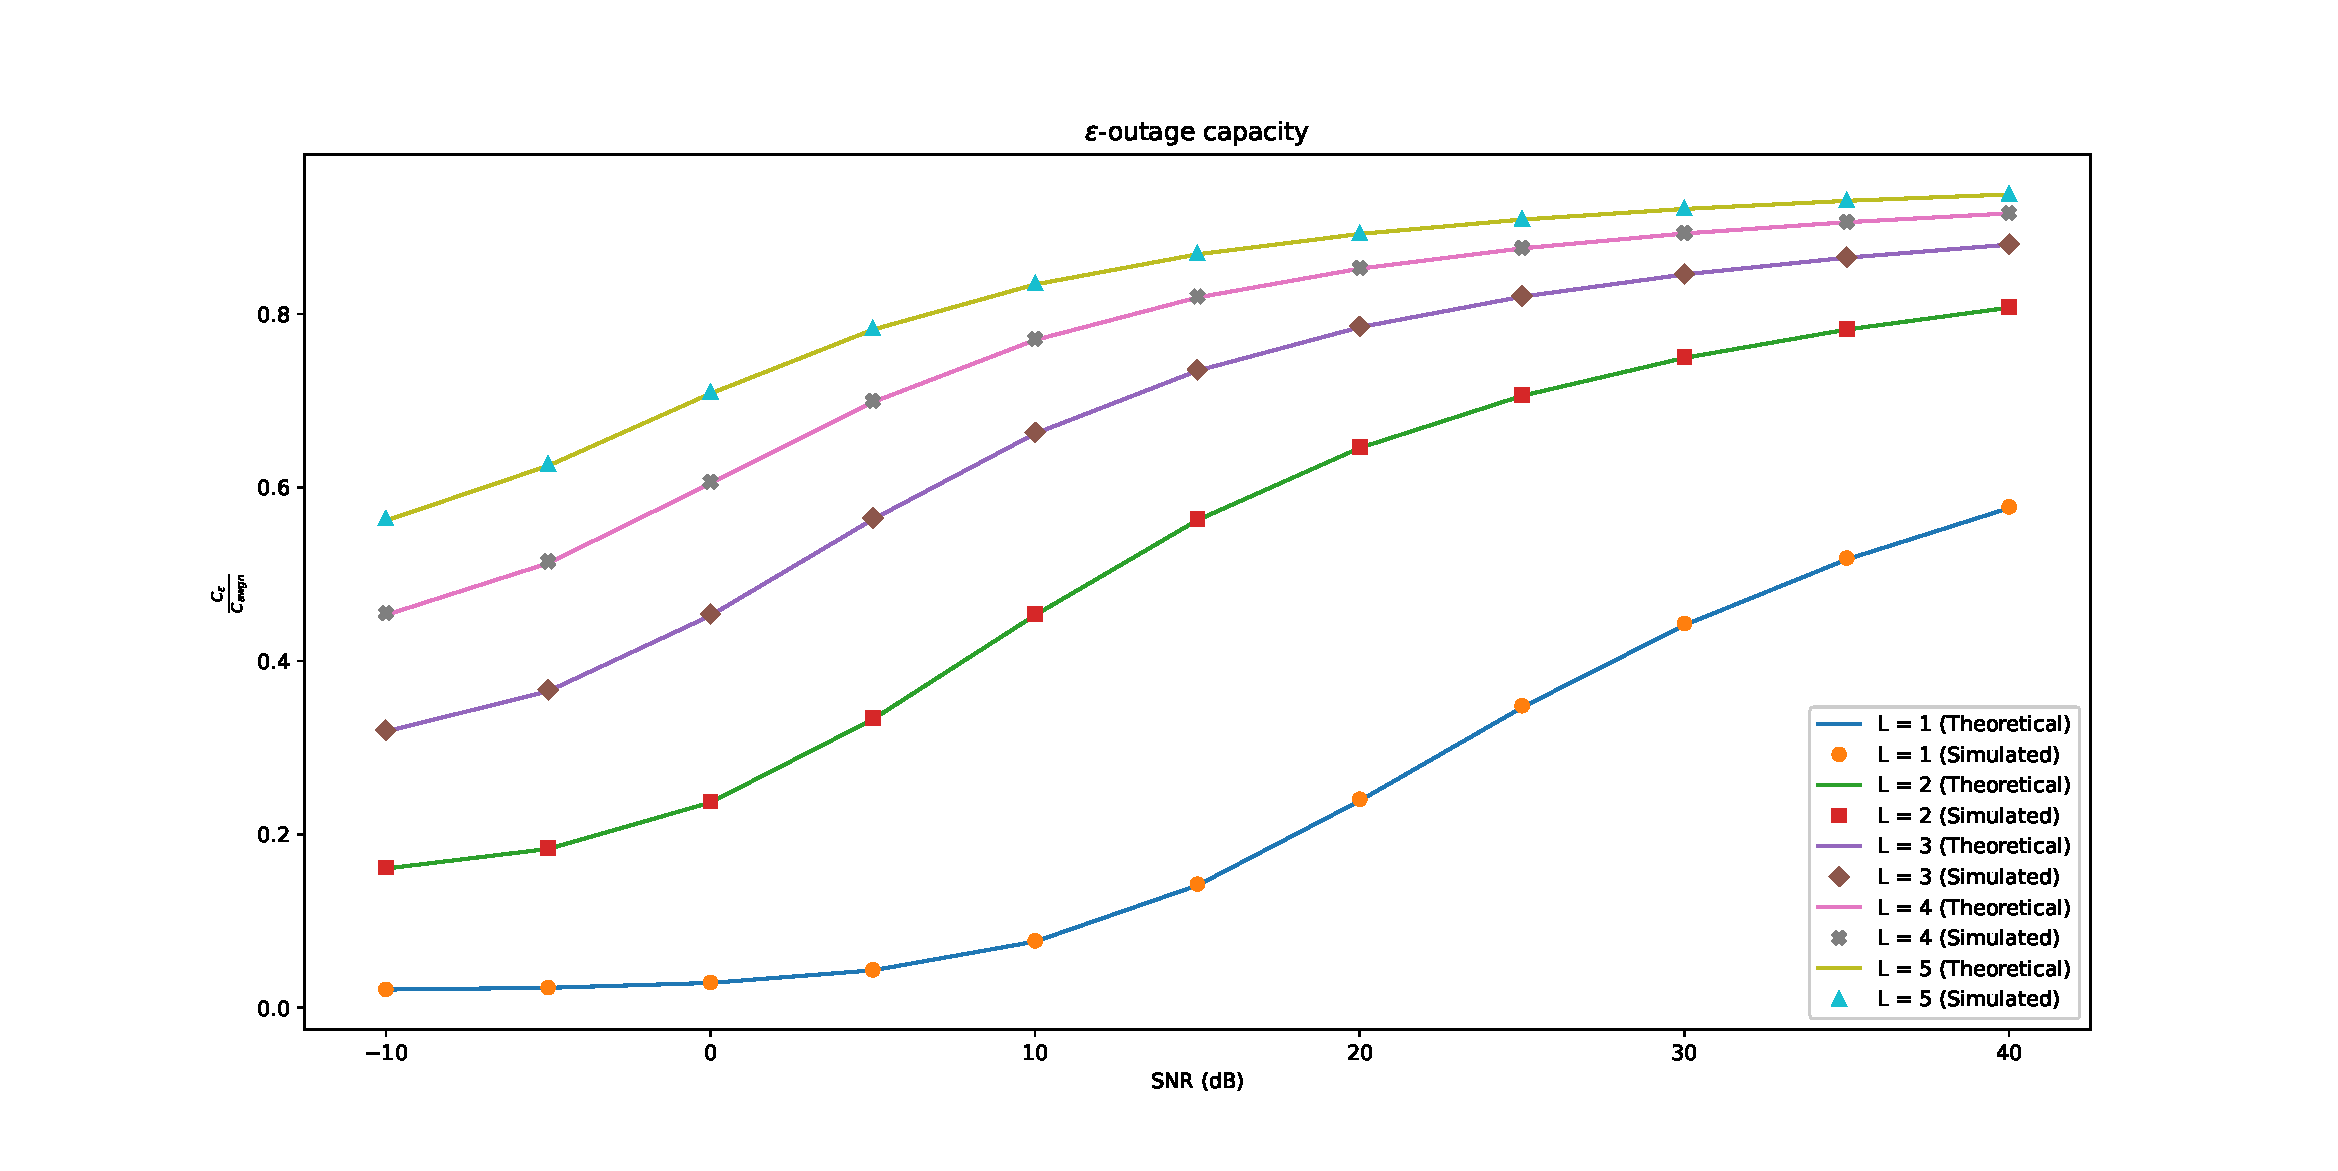
\includegraphics[scale = 0.85]{epsilon_outage.eps}
\end{figure}
  \end{enumerate}
\end{document}
